\section{Systemsicherheit unter iOS}
	Eine Reihe von aneinander gereihten und von einander abhängigen Prozessen
	trägt maßgeblich zur Systemsicherheit bei. Dies berücksichtigt vor allem den
	Startvorgang, die Software Updates - auch von Drittanbietern - und den Secure
	Enclave. Dies stellt sicher, dass alle Kernkomponenten, ob Hard- oder
	Software, möglichst gefeit vor Angriffen sind, ohne dabei die
	Nutzerfreundlichkeit zu beeinflussen. Nachfolgend werden die an
	diesem Prozess beteiligten Komponenten detailliert vorgestellt.
	%\begin{wrapfigure}[Zeilen]{Position}[Ueberhang]{Breite}
	%\begin{wrapfigure}[0]{r}[0.5cm]{6cm}
	\begin{wrapfigure}[3]{r}{6cm}
		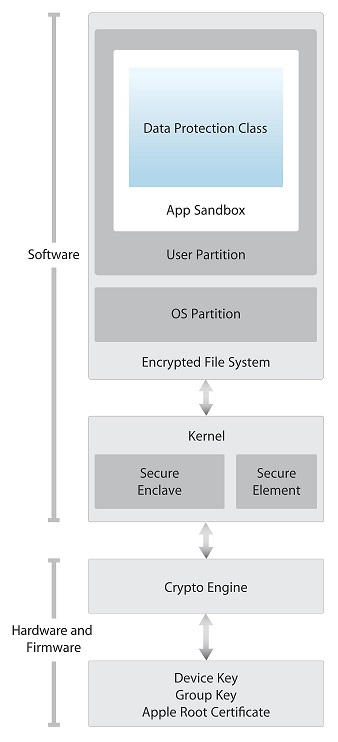
\includegraphics[width=\linewidth]{ios/media/security-model.jpg}
		\caption{Sicherheitsmodel von iOS}
		\label{fig:security-model}
	\end{wrapfigure}

	\subsection{Secure boot chain}
		Dieses Verfahren stellt eine Manipulation der \\
		Low-Level Software sicher. Nur iOS Geräte, \\
		die eine erfolgreiche Validierung dieser\\ 
		Vertrauenskette bestanden haben	starten\\ 
		ordnungsgemäß. Dabei wird nach dem Start\\
		eines iOS Gerätes zuerst Code aus einem nur lesbaren\\
		Speicherbereich ausgeführt. Dieser hardware of trust\\ 
		genannte und unveränderbare Code ist bei der\\
		Manufaktur der Chips eingebettet worden und somit\\
		implizit vertraulich. Das Boot ROM enthält zusätzlich\\
		Apple's öffentlichen Schlüssel des Wurzel-Zertifikats,\\
		welcher	sicher stellt, dass	der Low-Level-Bootloader\\
		von Apple signiert ist, bevor er ausgeführt wird.\\ 
		Dies ist der erste Schritt in der "`chain of trust"',\\ 
		in welcher jeder Teilnehmer sicher stellt,\\ 
		dass der darauf	folgende von Apple signiert	ist.
		
		%\begin{figure}[h]
			%\centering
	 		%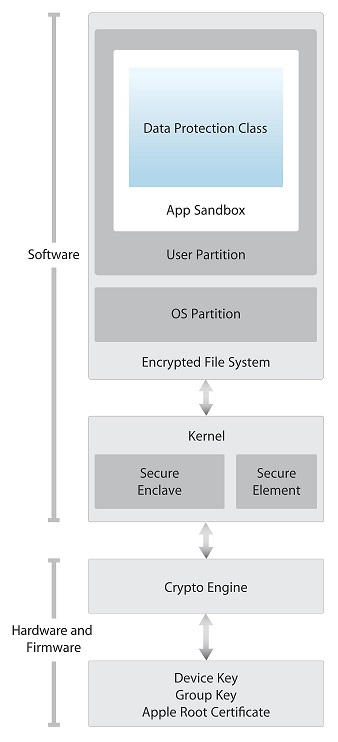
\includegraphics[width=0.3\linewidth]{ios/media/security-model.jpg}
	        %\caption{Sicherheitsarchitektur Diagramm von iOS}
	        %\label{fig:security-model}
	    %\end{figure}\\
	    %ref: Figure \ref{fig:security-model} shows the sec. arch.
	    
	    %\begin{wrapfigure}[Zeilen]{Position}[Ueberhang]{Breite}
		
	\subsection{Authorisierung von System Software}
		
	\subsection{iOS Sicherheitsmodel}
		Apple integrierte vier Schichten der Sicherheit in iOS.\\